\documentclass[french]{article}

\usepackage[utf8]{inputenc}
\usepackage[T1]{fontenc}
\usepackage{lmodern}
\usepackage[a4paper]{geometry}
\usepackage{babel}
\usepackage{hyperref}
\usepackage{array}
\usepackage{graphicx}

\title{Développement d'application \\ Projet : Wikipédia Matrix}
\date{Février 2020}
\author{Florian \textsc{Givernaud}, Nicolas \textsc{Sénave}}

\begin{document}

\large
\noindent

\maketitle

\textit{Enseignant} : Mathieu Acher

\section{Introduction}

Le but de se projet est d'extraire de façon automatisée des données provenant de tableaux Wikipédia. Il existe sur Wikipédia de nombreuses pages où figurent des tableaux, mais récupérer ces informations dans un format clair et réutilisable est difficile, à cause de la forme dans laquelle sont écrites les pages Wikipédia (\textit{html} ou \textit{Wikitext}) où se mêlent le contenu et la présentation, avec certes des conventions mais pas de norme parfaitement définie. La récupération de ces données n'est ainsi a priori pas facilement généralisable.\\

L'objectif est que la solution proposée ne se limite pas à un simple \textit{parser} aveugle, mais que cette solution fournisse également des indicateurs sur la qualité des informations extraites.

\section{Démarche}

\subsection{Technologies utilisées}

Nous avons travaillé à partir des pages Wikipédia lues au format \textit{html}.\\

Le format de sortie des données est le \textit{csv} ; ce format est très répandu, et encore largement utilisé et interprétable par de nombreux logiciels, langages, frameworks etc.\\

Le langage utilisé est Java, avec la librairie \textit{Jsoup} pour parser les pages web, la libraire \textit{OpenCSV} pour écrire les fichiers \textit{csv}, et \textit{CSVParser} pour tester la forme des csv en sortie.\\

Notre solution est accessible sur le répertoire git \url{https://github.com/nsenave/projet-wikimatrix}.

À la racine du dépôt figurent un \texttt{README.md} expliquant comment utiliser notre application, et un dossier "wikimatrix" qui est un projet Maven (les dépendances sont gérées via le \texttt{pom.xml}).

\subsection{Travail réalisé}

Le point de départ de notre travail a été d'importer le modèle proposé pour le projet sur le dépôt git \url{https://github.com/acherm/wikipediamatrix-bench}. Nous avons commencé en important les dépendances (Jsoup, CVSParser, OpenCSV, et Log4j) avec Maven via le pom.xml.

Nous n'auront pas utilisé Log4j, mais la librairie logging (java.util).\\

Les premiers essais ont été effectués dans une classe test SingleTest, où on n'essaye d'extraire les données que sur une seule page (\url{https://en.wikipedia.org/wiki/Comparison_of_Canon_EOS_digital_cameras}).

L'objectif était de se familiariser avec les APIs (Jsoup pour lire, OpenCSV pour écrire) et avec le format des données brutes. En effet le contenu dans les cellules du tableau peuvent ont des formes variées : le texte est parfois écrit dans un lien (balise \texttt{<a>}), ou dans une balise de mise en forme dont le contenu n'est pas toujours destiné à être affiché (\texttt{<span style:"display:none">} par exemple). \\

Nous avons implémenté deux parsers, qui ont été écrit à partir de cette première page. Le premier visa à récupérer le contenu le plus proprement possible, le second reprend le premier en intégrant un filtrage des tableaux parasites (par exemple le tableau contenant les références en bas de page, dont la forme est inexploitable dans notre démarche). Les résultats sont détaillés dans la partie suivante. \\

Ces parsers (classes Parser1 et Parser2), sont des implémentations d'une interface Parser. Cette implémentation correspond au \textbf{\textit{design pattern} Strategy}. L'interface mère contient la méthode principale \texttt{parseHtmlFromUrl} sous forme abstraite.

Cette méthode renvoie une liste d'éléments de la classe Tableau qui est un POJO (\textit{Plain old Java object}) destiné à contenir les informations des tableaux avant de les écrire dans des fichiers csv avec la classe TableauCSVWriter.

Une fois ces deux premiers parsers mis au point, nous avons lancé le test sur l'ensemble des urls figurant dans le fichier \texttt{input/wikiurls.txt}.

Nous avons enlevé deux liens de la liste originale : une des page contient le caractère spécial "\%" dans son url et provoque une erreur, une des pages a été supprimée.\\

Pour tester la qualité des sorties (bon nombre de colonnes, de lignes, en-têtes cohérent), nous souhaitions :
\begin{itemize}
	\item sélectionner un petit échantillon de pages sur lesquelles nous avons relevé manuellement ces informations, et les comparer avec celles des csv en sortie ;
	\item tester pour chaque url si ces informations sont cohérentes d'un parser à l'autre ;
	\item effectuer des tests standards sur le format des csv (nombre identique de colonnes sur chaque ligne etc.).
\end{itemize} 

La classe TableauCSVChecker propose des méthodes pour réaliser ces tests (en utilisant la libraire CSVParser). Cependant, par manque de temps, nous n'avons pas intégré cet outil dans les classes de test.

\subsection{Structure de l'application}

Le diagramme de classe ci-dessous présente schématiquement la structure de l'application :

\begin{figure}[h!]
	\centering
	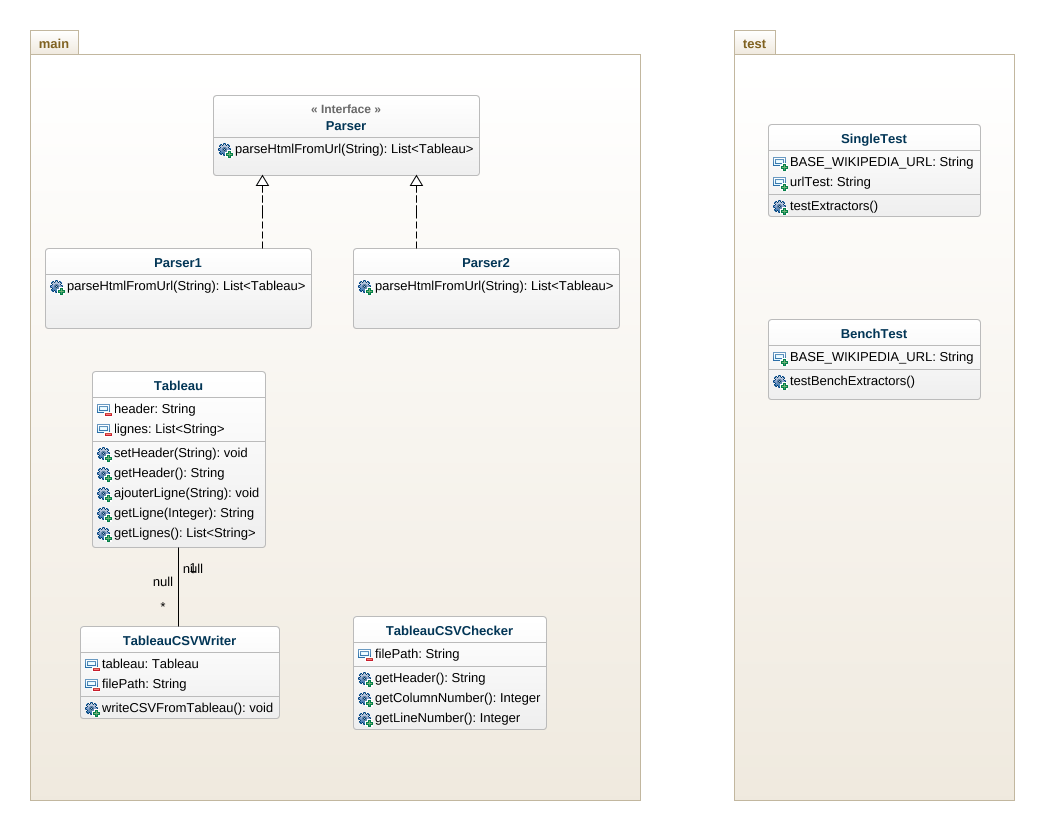
\includegraphics[width=\textwidth]{images/class-diagram.png}
	\caption{Diagramme de classes de l'application}
	\label{fig:class-diagram}
\end{figure}

\newpage

\section{Résultats}

Sur la page qui a été utilisée pour construire les parsers, nous arrivons à un résultat satisfaisant. Les nombres de lignes et colonnes sont corrects (69 et 19), et le contenu paraît proche de ce que l'on a sur la page d'origine.

Le deuxième extracteur filtre correctement deux tableaux parasites situés dans la section "Références" de la page.\\

Sur l'ensemble des autres pages, il existe plusieurs problèmes qui ne sont pas captés par les extracteurs. Par exemple une des causes qui amène à des sorties inexploitables est la présence de tableaux au sein d'un tableau, problème que nous n'avons pas su traiter.\\

Nous avons aussi une erreur "\textit{OutOfMemory Java heap space}" lors du lancement de l'application sur le banc d'essai complet, probablement à cause de la fonction \texttt{extractTextFromNode}  qui va chercher récursivement tout le contenu des balises \texttt{<td>}.

\section{Conclusion}

L'application réalisée pour ce projet propose un outil d'extraction des données tabulaires de Wikipédia. Cet outil ne donnera pas des résultats corrects sur 100\% des pages (le pourcentage de bons résultats est en l'état difficile à estimer), mais il constitue un premier pas dans ce but et pourrait être rendu plus robuste en élargissant le champ des cas de figures considérés dans les parsers.
	
\end{document}

